%%% LaTeX-Vorlage Version 1.8 %%%

% Grundlegende Dokumenteneigenschaften gemäß DHBW-Vorgaben
\documentclass[a4paper,fontsize=11pt,oneside,parskip=half,headings=normal]{scrreprt} 
% \usepackage{showframe} % nur für Kontrolle der Ränder 

%%% Präambel einbinden (mit Festlegungen gemäß DHBW-Vorgaben) %%%
%%% Präambel %%%
% hier sollten keine Änderungen erforderlich sein
%
\usepackage[utf8]{inputenc}   % Zeichencodierung UTF-8 für Eingabe-Dateien
\usepackage[T1]{fontenc}      % Darstellung von Umlauten im PDF

\usepackage{listings}         % für Einbindung von Code-Listings
\lstset{numbers=left,numberstyle=\tiny,numbersep=5pt,texcl=true}
\lstset{literate=             % erlaubt Sonderzeichen in Code-Listings 
{Ö}{{\"O}}1
{Ä}{{\"A}}1
{Ü}{{\"U}}1
{ß}{{\ss}}2
{ü}{{\"u}}1
{ä}{{\"a}}1
{ö}{{\"o}}1
{€}{{\euro}}1
}

\usepackage[
  inner=35mm,outer=15mm,top=25mm,
  bottom=20mm,foot=12mm,includefoot
]{geometry}                 % Einstellungen für Ränder

\usepackage[ngerman]{babel} % Spracheinstellungen Deutsch
\usepackage[babel,german=quotes]{csquotes} % deutsche Anf.zeichen
\usepackage{enumerate}      % anpassbare Nummerier./Aufz.
\usepackage{graphicx}       % Einbinden von Grafiken
\usepackage[onehalfspacing]{setspace} % anderthalbzeilig

\usepackage{blindtext}      % Textgenerierung für Testzwecke
\usepackage{color}          % Verwendung von Farbe 

\usepackage{acronym}        % für ein Abkürzungsverzeichnis

\usepackage[                % Biblatex
  backend=biber,
  bibstyle=_dhbw_authoryear,maxbibnames=99,
  citestyle=authoryear,     
  uniquename=true, useprefix=true,
  bibencoding=utf8]{biblatex}
%kein Punkt am Ende bei \footcite
%http://www.golatex.de/footcite-ohne-punkt-am-schluss-t4865.html
\renewcommand{\bibfootnotewrapper}[1]{\bibsentence#1}


%Reihenfolge der Autorennamen
%   
% http://golatex.de/viewtopic,p,80448.html#80448
% Argumente: siehe http://texwelt.de/blog/modifizieren-eines-biblatex-stils/
\DeclareNameFormat{sortname}{% Bibliographie
  \ifnum\value{uniquename}=0 % Normalfall
    \ifuseprefix%
      {%
         \usebibmacro{name:family-given}
           {\namepartfamily}
           {\namepartgiveni}
           {\namepartprefix}
           {\namepartsuffixi}%
       }
      {%
         \usebibmacro{name:family-given}
           {\namepartfamily}
           {\namepartgiveni}
           {\namepartprefixi}
           {\namepartsuffixi}%
       }%
  \fi
  \ifnum\value{uniquename}=1% falls nicht eindeutig, abgek. Vorname 
      {%
         \usebibmacro{name:family-given}
           {\namepartfamily}
           {\namepartgiveni}
           {\namepartprefix}
           {\namepartsuffix}%
       }%
  \fi
  \ifnum\value{uniquename}=2% falls nicht eindeutig, ganzer Vorname 
      {%
         \usebibmacro{name:family-given}
           {\namepartfamily}
           {\namepartgiven}
           {\namepartprefix}
           {\namepartsuffix}%
       }%
  \fi   
  \usebibmacro{name:andothers}}

\DeclareNameFormat{labelname}{% für Zitate
  \ifnum\value{uniquename}=0 % Normalfall
    \ifuseprefix%
      {%
         \usebibmacro{name:family-given}
           {\namepartfamily}
           {\empty}
           {\namepartprefix}
           {\namepartsuffixi}%
       }
      {%
         \usebibmacro{name:family-given}
           {\namepartfamily}
           {\empty}
           {\namepartprefixi}
           {\namepartsuffixi}%
       }%
  \fi
  \ifnum\value{uniquename}=1% falls nicht eindeutig, abgek. Vorname 
      {%
         \usebibmacro{name:family-given}
           {\namepartfamily}
           {\namepartgiveni}
           {\namepartprefix}
           {\namepartsuffix}%
       }%
  \fi
  \ifnum\value{uniquename}=2% falls nicht eindeutig, ganzer Vorname 
      {%
         \usebibmacro{name:family-given}
           {\namepartfamily}
           {\namepartgiven}
           {\namepartprefix}
           {\namepartsuffix}%
       }%
  \fi   
  \usebibmacro{name:andothers}}
      
  
\DeclareFieldFormat{extrayear}{% = the 'a' in 'Jones 1995a'
  \iffieldnums{labelyear}
    {\mknumalph{#1}}
    {\mknumalph{#1}}}        

\renewcommand*{\multinamedelim}{\addslash}
\renewcommand*{\finalnamedelim}{\addslash}
\renewcommand*{\multilistdelim}{\addslash}
\renewcommand*{\finallistdelim}{\addslash}

\renewcommand{\nameyeardelim}{~}

% Literaturverzeichnis: Doppelpunkt zwischen Name (Jahr): Rest 
% http://de.comp.text.tex.narkive.com/Tn1HUIXB/biblatex-authoryear-und-doppelpunkt
\renewcommand{\labelnamepunct}{\addcolon\addspace}

% damit die Darstellung für Vollzitate von Primärquellen in 
% Fußnoten später auf "nicht fett" geändert werden kann 
% (nur für Zitate von Sekundärliteratur relevant)
\newcommand{\textfett}[1]{\textbf{#1}}

% für Zitate von Sekundärliteratur:
\newcommand{\footcitePrimaerSekundaer}[4]{%
  \renewcommand{\textfett}[1]{##1}%
  \footnote{\fullcite[#2]{#1}, zitiert nach \cite[#4]{#3}}%  
  \renewcommand{\textfett}[1]{\textbf{##1}}%
}

% Im Literaturverzeichnis: Autor (Jahr) fett
\renewbibmacro*{author}{%
  \ifboolexpr{%
    test \ifuseauthor%
    and
    not test {\ifnameundef{author}}
  }
    {\usebibmacro{bbx:dashcheck}
       {\bibnamedash}
       {\usebibmacro{bbx:savehash}%
        \textfett{\printnames{author}}%
        \iffieldundef{authortype}
          {\setunit{\addspace}}
          {\setunit{\addcomma\space}}}%
     \iffieldundef{authortype}
       {}
       {\usebibmacro{authorstrg}%
        \setunit{\addspace}}}%
    {\global\undef\bbx@lasthash
     \usebibmacro{labeltitle}%
     \setunit*{\addspace}}%
  \textfett{\usebibmacro{date+extrayear}}}

% Sonderfall: Quelle ohne Autor, aber mit Herausgeber
% Name des Herausgebers wird fett gedruckt
\renewbibmacro*{bbx:editor}[1]{%
  \ifboolexpr{%
    test \ifuseeditor%
    and
    not test {\ifnameundef{editor}}
  }
    {\usebibmacro{bbx:dashcheck}
       {\bibnamedash}
       {\textfett{\printnames{editor}}%
        \setunit{\addcomma\space}%
        \usebibmacro{bbx:savehash}}%
     \usebibmacro{#1}%
     \clearname{editor}%
     \setunit{\addspace}}%
    {\global\undef\bbx@lasthash
     \usebibmacro{labeltitle}%
     \setunit*{\addspace}}%
  \textfett{\usebibmacro{date+extrayear}}}

% Anpassungen für deutsche Sprache
\DefineBibliographyStrings{ngerman}{%
	nodate = {{o.J.}},
	urlseen = {{Abruf:}},
	ibidem = {{ebenda}}
}

% keine Anführungszeichen beim Titel im Literaturverzeichnis
\DeclareFieldFormat[article,book,inbook,inproceedings,manual,misc,phdthesis,thesis,online,report]{title}{#1\isdot}

\newcommand{\literaturverzeichnis}{%
% nur Literaturverzeichnis
% (als eigenes Kapitel)
\phantomsection
\addcontentsline{toc}{chapter}{Literaturverzeichnis}
\spezialkopfzeile{Literaturverzeichnis}
\defbibheading{lit}{\chapter*{Literaturverzeichnis}}
\label{chapter:quellen}
\printbibliography[heading=lit,notkeyword=ausblenden]
} % mit DHBW-spezifischen Einstellungen

\usepackage{hyperref}       % URL-Formatierung, klickbare Verweise

\usepackage{tocloft}        % für Verzeichnis der Anhänge

\newcounter{anhcnt}
\setcounter{anhcnt}{0}
\newlistof{anhang}{app}{}

\newcommand{\anhang}[1]{%
  \refstepcounter{anhcnt}
  \setcounter{anhteilcnt}{0}
  \section*{Anhang \theanhcnt: #1}
  \addcontentsline{app}{section}{\protect\numberline{Anhang \theanhcnt}#1}\par
}

\newcounter{anhteilcnt}
\setcounter{anhteilcnt}{0}

\newcommand{\anhangteil}[1]{%
	\refstepcounter{anhteilcnt}
	\subsection*{Anhang~\arabic{anhcnt}/\arabic{anhteilcnt}: #1}
	\addcontentsline{app}{subsection}{\protect\numberline{Anhang \theanhcnt/\arabic{anhteilcnt}}#1}\par
}

\renewcommand{\theanhteilcnt}{Anhang \theanhcnt/\arabic{anhteilcnt}}

% vgl. S. 4 Paket-Beschreibung tocloft 	
% Einrückungen für Anhangverzeichnis
\makeatletter
\newcommand{\abstaendeanhangverzeichnis}{
\renewcommand*{\l@section}{\@dottedtocline{1}{0em}{5.5em}}
\renewcommand*{\l@subsection}{\@dottedtocline{2}{2.3em}{6.5em}}
}
\makeatother

% Abbildungs- und Tabellenverzeichnis
% Bezeichnungen
\renewcaptionname{ngerman}{\figurename}{Abb.}
\renewcaptionname{ngerman}{\tablename}{Tab.}
% Einrückungen
\makeatletter
\renewcommand*{\l@figure}{\@dottedtocline{1}{0em}{2.3em}}
\renewcommand*{\l@table}{\@dottedtocline{1}{0em}{2.3em}}
\makeatother


\usepackage{chngcntr}                % fortlaufende Zähler für Fußnoten, Abbildungen und Tabellen
\counterwithout{figure}{chapter}
\counterwithout{table}{chapter}
\counterwithout{footnote}{chapter}

\usepackage[automark]{scrlayer-scrpage} 
%% Definitionen für Kopf- und Fußzeile auf normalen Seiten
\defpagestyle{kopfzeile}
{% Kopfdefinition
  (\textwidth,0pt)    % Länge der oberen Linie,Dicke der oberen Linie       
  {} % Definition für linke Seiten im doppelseitigen Layout
  {} % Definition für rechte Seiten im doppelseitigen Layout      
  {  % Definition für Seiten im einseitigen Layout
	\makebox[0pt][l]{\rightmark}% 
	\makebox[\linewidth]{}% 
  }        
  (\textwidth, 0.4pt) % Untere Linienlänge, Untere Liniendicke
}
{% Fußdefinition
  (\textwidth,0pt)    % Obere Linienlänge, Obere Liniendicke
  {} % Definition für linke Seiten im doppelseitigen Layout
  {} % Definition für rechte Seiten im doppelseitigen Layout
  {  % Definition für Seiten im einseitigen Layout
    \makebox[\linewidth]{}%
    \makebox[0pt][r]{\pagemark}%
  }
  (\textwidth, 0pt)   % Länge der unteren Linie,Dicke der unteren Linie
}

%% Definitionen für Kopf- und Fußzeile auf ersten Seiten eines Kapitels
\defpagestyle{kapitelkopfzeile}
{% Kopfdefinition
  (\textwidth,0pt)    % Länge der oberen Linie,Dicke der oberen Linie       
  {} % Definition für linke Seiten im doppelseitigen Layout
  {} % Definition für rechte Seiten im doppelseitigen Layout      
  {}  % Definition für Seiten im einseitigen Layout
  (\textwidth, 0pt) % Untere Linienlänge, Untere Liniendicke
}
{% Fußdefinition
  (\textwidth,0pt)    % Obere Linienlänge, Obere Liniendicke
  {} % Definition für linke Seiten im doppelseitigen Layout
  {} % Definition für rechte Seiten im doppelseitigen Layout
  {  % Definition für Seiten im einseitigen Layout
    \makebox[\linewidth]{}%
    \makebox[0pt][r]{\pagemark}%
  }
  (\textwidth, 0pt)   % Länge der unteren Linie,Dicke der unteren Linie
}

%% Definitionen für Kopf- und Fußzeile im Anhang und bei Quellenverzeichnisse
\newcommand{\spezialkopfzeileBezeichnung}{}
\defpagestyle{spezialkopfzeile}
{% Kopfdefinition
  (\textwidth,0pt)    % Länge der oberen Linie,Dicke der oberen Linie       
  {} % Definition für linke Seiten im doppelseitigen Layout
  {} % Definition für rechte Seiten im doppelseitigen Layout      
  {  % Definition für Seiten im einseitigen Layout
	\makebox[0pt][l]{\spezialkopfzeileBezeichnung}% 
	\makebox[\linewidth]{}% 
  }        
  (\textwidth, 0.4pt) % Untere Linienlänge, Untere Liniendicke
}
{% Fußdefinition
  (\textwidth,0pt)    % Obere Linienlänge, Obere Liniendicke
  {} % Definition für linke Seiten im doppelseitigen Layout
  {} % Definition für rechte Seiten im doppelseitigen Layout
  {  % Definition für Seiten im einseitigen Layout
    \makebox[\linewidth]{}%
    \makebox[0pt][r]{\pagemark}%
  }
  (\textwidth, 0pt)   % Länge der unteren Linie,Dicke der unteren Linie
}
            
\newcommand\spezialkopfzeile[1]{%
  \renewcommand\spezialkopfzeileBezeichnung{#1}
  \pagestyle{spezialkopfzeile}
}
                
% Standard-Pagestyle auswählen
\pagestyle{kopfzeile}

% keine Kopfzeile anzeigen auf Seiten, auf denen ein 
% Kapitel beginnt oder das Inhalts-/Abbildungs-/Tabellenverzeichnis steht 
\renewcommand{\chapterpagestyle}{kapitelkopfzeile}
\tocloftpagestyle{kapitelkopfzeile}

		 % für schöne Kopfzeilen 

\usepackage{textcomp}            % erlaubt EUR-Zeichen in Eingabedatei
\usepackage{eurosym}             % offizielles EUR-Symbol in Ausgabe
\renewcommand{\texteuro}{\euro}  % ACHTUNG: nach hyperref aufrufen!

\usepackage{scrhack}             % stellt Kompatibilität zw. KOMA-Script
                                 % (scrreprt) und anderen Paketen her

\usepackage{float}
                                 
% Anpassung der Abstände bei Kapitelüberschriften
% (betrifft auch Inhalts-, Abbildungs- und Tabellenverzeichnis)
\renewcommand*\chapterheadstartvskip{\vspace*{-\topskip}}
\newcommand{\myBeforeTitleSkip}{1mm}
\newcommand{\myAfterTitleSkip}{10mm}
\setlength\cftbeforetoctitleskip{\myBeforeTitleSkip}
\setlength\cftbeforeloftitleskip{\myBeforeTitleSkip}
\setlength\cftbeforelottitleskip{\myBeforeTitleSkip}

\setlength\cftaftertoctitleskip{\myAfterTitleSkip}
\setlength\cftafterloftitleskip{\myAfterTitleSkip}
\setlength\cftafterlottitleskip{\myAfterTitleSkip}                                                            
%%% Ende der Präambel %%%

%%% Name der eigenen Literatur-Datenbank (ggf. anpassen) %%%
\bibliography{includes/Wiss-Ausarbeitung.bib}

\begin{document}
%%% Deckblatt einbinden %%% 
% Anpassungen nötig (Name, Titel etc.)
% HIER EDITIEREN: 
% Typ der Arbeit (für Deckblatt und Metadaten)
% - bitte Zutreffendes auswählen
%\newcommand{\typMeinerArbeit}{1. Projektarbeit} 
%\newcommand{\typMeinerArbeit}{2. Projektarbeit} 
%\newcommand{\typMeinerArbeit}{Seminararbeit} 
\newcommand{\typMeinerArbeit}{Projekt / Integrationsseminar} 

% Thema der Arbeit (für ehrenwörtliche Erklärung, ohne Umbrüche)
% HIER EDITIEREN: 
\newcommand{\themaMeinerArbeit}{Erstellung eines Wissensquiz für die Einführung von RAPLA an der DHBW Stuttgart}

% Vorname, Name der Autorin/des Autors (für Titelseite und Metadaten)
% HIER EDITIEREN:
\newcommand{\meinNameSB}{Simon Burbiel}
\newcommand{\meinNameLG}{Lukas Großerhode}
\newcommand{\meinNameSS}{Simon Spitzer}
\newcommand{\meinNameTK}{Tim Keicher}
\newcommand{\meinNameDS}{David Stark}

\thispagestyle{empty}

\begin{spacing}{1}
\begin{center}	
~\vspace{0mm}

% HIER EDITIEREN: Titel der Arbeit
{\sffamily
\LARGE  
% \Large  % bei sehr langen Titeln ggf. etwas kleinere Schriftart wählen
\textbf{Erstellung eines Wissensquiz für die Einführung von RAPLA an der DHBW Stuttgart}

% \bigskip
% \textbf{ggf. etwas länger}
}


\vspace{15mm}

% Typ wird automatisch eingefügt (oben festlegen)
{\Large \typMeinerArbeit}

\vspace{1cm}

% HIER ggf. EDITIEREN
vorgelegt am \today 

\vspace{15mm}

Fakultät Wirtschaft und Gesundheit
\medskip

Studiengang Wirtschaftsinformatik
\medskip

% HIER EDITIEREN: Kurs eintragen
Kurs WWI2021F 

\vspace{10mm}

von

\vspace{10mm}

% Vorname und Name wird automatisch eingefügt (oben festlegen) 
{\large\textsc{\meinNameSB}}
\medskip

{\large\textsc{\meinNameLG}}
\medskip

{\large\textsc{\meinNameTK}}
\medskip

{\large\textsc{\meinNameSS}}
\medskip

{\large\textsc{\meinNameDS}}
\medskip

\vspace{10mm}
\end{center}

\vfill




\vspace{1cm}
%(etwas Platz für die Unterschrift der Betreuerin/des Betreuers aus der Ausbildungsstätte)
\end{spacing}

% falls ein Vertraulichkeitsvermerk erforderlich ist,
% die Kommentarzeichen in den nachfolgenden Zeilen entfernen:
 
%\begin{center}
%\small
%\textbf{Vertraulichkeitsvermerk}:
%Der Inhalt dieser Arbeit darf weder als Ganzes noch in Auszügen \\
%Personen außerhalb des Prüfungs- und Evaluationsverfahrens zugänglich gemacht werden, sofern keine anders lautende Genehmigung des Dualen Partners vorliegt. 
%\end{center}

% Meta-Daten für PDF-Datei basierend auf obigen Angaben
\hypersetup{pdftitle={\themaMeinerArbeit}}
\hypersetup{pdfauthor={\meinNameLG}}
\hypersetup{pdfsubject={\typMeinerArbeit\ DHBW Stuttgart \the\year}}

%%% Umstellung der Seiten-Nummerierung auf i, ii, iii ... %%%
\pagenumbering{Roman}

%%% Abstract einbinden (optionale Kurzfassung Ihrer Arbeit) %%%
% \begin{abstract}
\thispagestyle{kapitelkopfzeile}
\textbf{\LaTeX-Vorlage für Projekt-, Seminar- und Bachelorarbeiten}

Bei dem vorliegenden Dokument handelt es sich um eine Vorlage, die
für Projekt-, Seminar- und Bachelorarbeiten im Studiengang
Wirtschaftsinformatik der DHBW Stuttgart verwendet werden kann.

Sie setzt die technischen Vorgaben der Zitierrichtlinien\footnote{Sie finden diese unter \enquote{Prüfungsleistungen} im Studierendenportal (\url{https://www.dhbw-stuttgart.de/studierendenportal/wirtschaftsinformatik/pruefungsleistungen/projekt-/bachelorarbeit/}).} des Studiengangs
(Stand: 07/2023) um.

\emph{Hinweise:} Bitte lesen Sie sich die Zitierrichtlinien unbedingt genau durch. Dieses Dokument ersetzt keine Anleitung oder Einführung in \LaTeX,
für die Nutzung sind daher gewisse Vorkenntnisse unerlässlich. Ein Einstieg in 
\LaTeX\ ist aber weniger schwierig, als es vielleicht auf den ersten Blick scheint
und lohnt sich für das Verfassen wissenschaftlicher Arbeiten in jedem Fall.\footnote{%
so auch \url{http://www.spiegel.de/netzwelt/tech/textsatz-keine-angst-vor-latex-a-549509.html}} 
Als Hilfestellung beim Schreiben eines Dokuments habe ich einen zweiseitigen kompakten \LaTeX-Spickzettel erstellt, der über Moodle verfügbar ist.

Ihre Rückmeldungen und Anregungen zu dieser Vorlage nehme ich gerne per E-Mail an die Adresse
\url{tobias.straub@dhbw-stuttgart.de} entgegen.

--- Prof. Dr. Tobias Straub

\vspace{5em}

\begin{center}\small
\begin{tabular}{ccl}
\multicolumn{3}{c}{\textbf{Versionshistorie}}\\
\hline
1.0	& 05.02.2015 & erste Fassung \\
\hline
1.1 & 16.02.2015 & siehe~\ref{anhang:ReleaseNotes11} \\
\hline
1.2 & 20.04.2015 & siehe~\ref{anhang:ReleaseNotes12} \\
\hline
1.3 & 20.02.2016 & siehe~\ref{anhang:ReleaseNotes13} \\
\hline
1.4 & 24.07.2017 & siehe~\ref{anhang:ReleaseNotes14} \\
\hline
1.5 & 07.01.2018 & siehe~\ref{anhang:ReleaseNotes15} \\
\hline
1.6 & 07.04.2018 & siehe~\ref{anhang:ReleaseNotes16} \\
\hline
1.7 & 12.02.2019 & siehe~\ref{anhang:ReleaseNotes17} \\
\hline
1.8 & 10.02.2020 & siehe~\ref{anhang:ReleaseNotes18} \\
\hline
1.9 & 19.07.2023 & siehe~\ref{anhang:ReleaseNotes19} \\
\end{tabular}
\end{center}

\end{abstract}


\cleardoublepage

%%% Inhalts-, Abbildungs-, Tabellenverzeichnisse %%%
% sollen einzeilig gesetzt werden, um Platz zu sparen 
\begin{spacing}{1}
\tableofcontents
\clearpage
\chapter*{Abkürzungsverzeichnis}
\addcontentsline{toc}{chapter}{Abkürzungsverzeichnis}

\begin{acronym}[RAPLA] 
% Argument definiert die Breite der ersten Spalte anhand des längsten vorkommenden Eintrags
\acro{DHBW}{Duale Hochschule Baden-Württemberg}
\acro{DIN}{Deutsches Institut für Normung}
\acro{ERP}{Enterprise-Resource-Planning}
\acro{MVP}{Minimum Viable Product}
\acro{PM}{Personenmonate}
\acro{RACI}{Responsible, Accountable, Consulted, Informed}
\acro{RAPLA}{Raumplanungsassistent}
\end{acronym}

\clearpage
\thispagestyle{kapitelkopfzeile}
\listoffigures
\phantomsection
\addcontentsline{toc}{chapter}{Abbildungsverzeichnis} % Abb.verz. ins Inh.verz. aufnehmen

\clearpage
\listoftables
\phantomsection
\addcontentsline{toc}{chapter}{Tabellenverzeichnis}   % Tab.verz. ins Inh.verz. aufnehmen
\end{spacing}

%%% Umstellung der Seiten-Nummerierung auf 1, 2, 3 ... %%%
\cleardoublepage
\pagenumbering{arabic}

%%% Ihr eigentlicher Inhalt %%%
% Empfehlung: strukturieren Sie Ihren Text in einzelnen Dateien 
% und binden Sie diese hier mit \input{includes/dateiname.tex} ein

\chapter{Einleitung}
\section{Motivation}
Bei der Einführung neuer Systeme in einem unternehmerischen oder universitären
Kontext ist die Schulung der Endbenutzerinnen und -benutzer ein zentraler Erfolgsfaktor.
\section{Problemstellung}
\section{Zielsetzung}
\section{Vorgehensweise}
\section{Aufbau der Arbeit}


% Die Einführung neuer Systeme und Prozesse erfordert
% stets eine umsichtige und durchdachte Herangehensweise. Diese beginnt bereits
% bei der Systemplanung und erstreckt sich über die Entwicklung bis hin zur abschließenden Migration.
% \footcite[Vgl.][S. 882 ff.]{laudonWirtschaftsinformatikEinfuehrung2016}
% Oftmals kommt es hierbei in der praktischen Umsetzung jedoch zu Fehlern, durch welche die geplante Einführung
% des jeweiligen Systems schlussendlich entweder stark verzögert oder sogar gar nicht stattfindet. Als Beispiel
% hierfür lässt sich die Implementierung eines neuen „\ac{ERP}“-Systems anführen. Auf einer Konferenz für \ac{ERP} benennen
% Becker und Winkelmann 2008 die fehlende Schulung von Mitarbeitenden als zentralen Faktor für das Scheitern eines solchen Projektes.
% \footcite[Vgl.][27]{becker10MoglichkeitenERPProjekt2008}
% Für die erfolgreiche Migration auf ein neues System sei es daher unabdingbar, die Endbenutzerinnen und -benutzer hinsichtlich der
% Bedienung und Funktionen zu schulen, um ein Scheitern der neuen Plattform oder Anwendung und damit eine Vergeudung monetärer und zeitlicher Ressourcen zu vermeiden.  
% \footcite[Vgl.][886]{laudonWirtschaftsinformatikEinfuehrung2016}

% Auch in der Fakultät Wirtschaft an der \acs{DHBW} Stuttgart soll im Jahr 2024 ein neues System eingeführt werden.
% Konkret handelt es sich hierbei um den zentralen Raumplanungsassistenten \acs{RAPLA}, welcher Studiengangsleiterinnen
% und -leiter sowie die zugehörigen Sekretariate bei der Buchung von Räumen unterstützen soll. Bislang erfolgt die Buchung von
% Räumen in der Fakultät Wirtschaft über Excel-Tabellen, wodurch ein sehr hoher Abstimmungsaufwand unter den Studiengängen
% hinsichtlich der effizientesten Belegung von Seminarräumen besteht. Diesem Aspekt kommt insbesondere in Anbetracht einer
% allgemeinen Raumknappheit der Hochschule eine hohe Bedeutung zu. Da \acs{RAPLA} jedoch noch nicht an allen Standorten im Einsatz ist,
% fehlt bislang in vielen Studienzentren das Wissen über den Aufbau, die Beschaffenheit sowie die Funktionen der Anwendung.

% Gegenwärtig wird daher ein statisches Schulungsdokument erstellt, durch welches den jeweiligen Studienzentren sowie Angehörigen der \acs{DHBW} Stuttgart
% bei der Einführung des Raumplanungsassistenten relevante Informationen zur Verfügung gestellt werden.
% Um den Teilnehmerinnen und Teilnehmern der Schulung einen möglichst hohen
% Mehrwert und einen intuitiven Einstieg in die Anwendung zu bieten, soll als Eigenleistung im Rahmen der Projektkonzeption ergänzend zu
% der bereits bestehenden Schulungsdokumentation ein Wissensquiz entwickelt werden, welches direkt in Moodle abgebildet sein wird.
% Dieses soll die Nutzerinnen und Nutzer dazu motivieren, sich mit Anwendung aktiv zu beschäftigen und sie zum Lernen und Ausprobieren
% anregen. Den erfolgreichen Abschluss des Kurses bildet eine persönliche Zertifizierung, welche den Teilnehmenden digital
% zur Verfügung gestellt wird. Die Umsetzung in Moodle wird erreicht, indem in einem ersten Schritt eine umfassende Analyse der Gegebenheiten erfolgt, zu denen bspw.
% die Ziel- und Interessengruppen, vor- und nachgelagerte Prozesse sowie das Programm selbst gehören. Zusätzlich werden die gegenwärtigen
% Schulungsunterlagen gesichtet und die Funktionsfähigkeit von \acs{RAPLA} mittels eines Testzugangs untersucht. Darauf aufbauend wird
% in einem zweiten Schritt eine Seite in Moodle erstellt, auf welcher das Wissensquiz abgebildet sein wird. Im dritten
% Schritt erfolgt eine Evaluation des neuen Schulungsprozesses, welcher eine empirische Validierung mit echten Anwenderinnen und
% Anwendern vorausgeht. Anhand dieser Evaluation soll abschließend hervorgehen, ob und inwiefern die Moodle-Zertifizierung vorteilhaft
% für den operativen Einsatz ist und welche Änderungen und Ergänzungen darauf aufbauend für zukünftige Aktualisierungen in Betracht zu ziehen sind.

% ----


% Daher soll im Rahmen der Studienfächer „Projektkonzeption“, „Projekt“ und „Integrationsseminar“ ein Schulungskonzept erstellt
% werden, welches die jeweiligen Studienzentren sowie Angehörigen der DHBW Stuttgart bei der erfolgreichen Einführung von \acs{RAPLA}
% unterstützt. Dies wird erreicht, indem in einem ersten Schritt eine umfassende Analyse der Gegebenheiten erfolgt, zu denen bspw.
% die Ziel- und Interessengruppen, vor- und nachgelagerte Prozesse sowie das Programm selbst gehören. Zusätzlich werden die gegenwärtigen
% Schulungsunterlagen gesichtet und die Funktionsfähigkeit von \acs{RAPLA} mittels eines Testzugangs untersucht. Darauf aufbauend wird
% in einem zweiten Schritt ein vollumfängliches Schulungskonzept inklusive Schulungsunterlagen erstellt, das Auskunft darüber gibt,
% welche Personenkreise zu welchem Zeitpunkt mit welchen Mitteln zu schulen sind, um das jeweilige Ziel zu erreichen. Im dritten
% Schritt erfolgt eine Evaluation des neuen Schulungsprozesses, welcher eine empirische Validierung mit echten Anwenderinnen und
% Anwendern vorausgeht. Anhand dieser Evaluation soll abschließend hervorgehen, ob und inwiefern das neue Konzept vorteilhaft
% für den operativen Einsatz ist und welche neuen Funktionen darauf aufbauend für zukünftige Aktualisierungen in Betracht zu ziehen sind.


\chapter{Theoretischer Hintergrund}
\section{E-Learning und digitale Wissensvermittlung}
\section{Didaktische Konzepte für die Wissensquiz-Erstellung}
\section{Zertifizierungen als Erfolgsfaktor}
\section{RAPLA 2.0 als Prüfungsgegenstand}


Das ist ein Test.
\chapter{Projektbeschreibung}
% noch mal Bezug nehmen auf das Projektplanungsdokument (nur das, was wirklich relevant
% für dieses Projekt ist)
\section{Ausgangslage und Problemstellung}
Die Ausgangslage dieses Projektes lässt sich durch die dringende Notwendigkeit einer umfassenden Schulung sowie einer anschließenden Zertifizierung zur Einführung des neuen Raumplanungsassistenten RAPLA beschreiben. Dieser Assistent soll den Prozess der Raumplanung erheblich vereinfachen und optimieren. Für die erfolgreiche Einführung ist es jedoch unerlässlich, dass die Nutzerinnen und Nutzer entsprechend geschult und zertifiziert werden. Im Rahmen dieser Gruppenarbeit liegt der organisatorische Schwerpunkt auf der Implementierung der Zertifizierung. Diese wird durch die Entwicklung eines Wissensquizzes und eines abschließenden Zertifizierungsquizzes realisiert. Das zugrunde liegende Projektplanungsdokument hebt hervor, dass die inhaltliche Komplexität des Raumplanungsassistenten RAPLA eine tiefgehende und umfassende Schulung sowie eine präzise Zertifizierung notwendig macht. Daher ist eine strukturierte und detaillierte Herangehensweise erforderlich, um sicherzustellen, dass alle relevanten Aspekte abgedeckt werden und die Nutzerinnen und Nutzer optimal vorbereitet sind.

\section{Anforderungen an das Quiz}
Die Anforderungen an das Quiz sind äußerst vielfältig und umfangreich. Zum einen soll das Quiz die Lernenden auf die bevorstehende Zertifizierung optimal vorbereiten, wobei ein besonderer Fokus auf einer hohen Benutzerfreundlichkeit liegt. Dies bedeutet, dass das Quiz intuitiv und einfach zu bedienen sein muss, um eine positive Lernerfahrung zu gewährleisten. Zum anderen dient das Quiz der Überprüfung des erworbenen Wissens in Bezug auf den gesamten Projektumfang. Hierbei ist es essenziell, dass das Quiz sowohl theoretische Fragen als auch praktische Aufgaben in unterschiedlichen Schwierigkeitsgraden enthält. Diese Fragen und Aufgaben müssen so formuliert sein, dass sie klare und eindeutige Antworten ermöglichen, was eine automatisierte Bewertung erleichtert. Nach der Bewertung soll den Lernenden eine Rückmeldung in Form eines Zertifikates gegeben werden, welches ihren Kenntnisstand offiziell bestätigt.
Für die Umsetzung des Quizzes wird die Lernplattform Moodle genutzt, da diese Plattform zahlreiche Funktionen bietet, die für die Erstellung und Durchführung eines interaktiven und effektiven Quizzes notwendig sind. Moodle ermöglicht es, verschiedene Fragetypen und Aufgabenformate zu integrieren, was zur Vielseitigkeit und Dynamik des Quizzes beiträgt. Darüber hinaus werden zwei reale Rapla-Instanzen zur Darstellung der Aufgaben verwendet. Insgesamt soll das Quiz nicht nur ein hohes Maß an Interaktivität bieten, sondern auch sicherstellen, dass die Lernenden intensiv mit den Inhalten des Raumplanungsassistenten RAPLA vertraut gemacht werden und so bestens auf die Zertifizierung vorbereitet sind.

\section{Methodik und Vorgehensweise}
Die Methodik und Vorgehensweise zur Umsetzung dieses Projektes ist in mehrere Phasen unterteilt, um eine systematische und strukturierte Herangehensweise zu gewährleisten.
In der Projektplanungsphase werden zunächst die Ziele und Aufgaben klar definiert. Ein detaillierter Zeitplan wird erstellt, der die verschiedenen Meilensteine des Projektes festlegt. Hierzu gehören unter anderem die Analyse, das Design, die Implementierung, das Testen und die finale Evaluierung.
Während der Analysephase wird eine umfassende Bedarfsanalyse durchgeführt, um die spezifischen Anforderungen an das Quiz zu ermitteln. Dies umfasst die Identifizierung der zu vermittelnden Inhalte sowie die Festlegung der Kriterien für die Zertifizierung. Die Anforderungsanalyse hilft dabei, die notwendigen Funktionalitäten und Eigenschaften des Quizzes zu bestimmen.
In der Designphase wird ein detailliertes Konzept für das Quiz entwickelt. Dies beinhaltet sowohl die inhaltliche Gestaltung als auch die Benutzeroberfläche. Das Ziel ist es, ein benutzerfreundliches und interaktives Quiz zu entwerfen, das den Lernenden eine effektive Vorbereitung ermöglicht.
Die Implementierungsphase umfasst die tatsächliche Programmierung des Quizzes. Dabei wird das Quiz in die Lernplattform Moodle integriert, die aufgrund ihrer vielseitigen Funktionen und Benutzerfreundlichkeit ausgewählt wurde. In dieser Phase werden die verschiedenen Fragetypen und Aufgabenformate erstellt und in das System eingebunden.
In der anschließenden Testphase wird das Quiz ausführlich getestet. Hierbei liegt der Fokus auf der Benutzerfreundlichkeit und der Funktionalität. Fehler und Probleme werden identifiziert und behoben, um sicherzustellen, dass das Quiz reibungslos funktioniert.
Die Evaluierung und Feedback-Phase beinhaltet das Sammeln von Rückmeldungen der ersten Nutzer. Basierend auf diesem Feedback werden notwendige Anpassungen vorgenommen, um die Qualität und Effektivität des Quizzes weiter zu verbessern.
In der letzten Phase, der Finalisierung und Rollout, wird die Abschlussdokumentation erstellt und das Quiz finalisiert. Zudem erfolgt der offizielle Rollout des Quizzes für alle Nutzer.
Diese strukturierte Vorgehensweise stellt sicher, dass das Projekt methodisch und effizient umgesetzt wird, wodurch die Ziele der Schulung und Zertifizierung des Raumplanungsassistenten RAPLA erfolgreich erreicht werden können.



\chapter{Konzeption des Wissensquiz}
\section{Analyse der vorhandenen Schulungsunterlagen}
\section{Erstellung und Aufbau des Fragenkatalogs}
\section{Darlegung des Prüf- und Freigabeprozesses}
% Gegenstand der Arbeitspaketeplanung ist die Struktur von Projekten hinsichtlich ihrer Komplexität.
% \footcite[Vgl.][128]{kusterHandbuchProjektmanagementAgil2022}
% Dies geschieht durch die Unterteilung des Projektes in kleinere Einheiten sowie durch die Erstellung eines Projektstrukturplans.
% Oftmals wird dieser einschließlich seiner Meilensteine auf Arbeitspaketebene aufgeteilt und somit für Projektmitarbeiter editierbar gemacht.
% \footcite[Vgl.][121]{panagosToolsUndMassnahmen2019}
% Dies ist vergleichbar mit einer umgekehrten Baumstruktur, bei welcher im oberen Bereich der jeweilige Meilenstein dargestellt ist und die Blätter die
% zugehörigen Arbeitspakete repräsentieren.
% \footcite[Vgl.][29]{kusay-merkleAgilesProjektmanagementIm2018}
% Im unteren Bereich sind schlussendlich die unteilbaren Arbeitspakete zu finden. In der Theorie können diese jedoch auf einer beliebigen Ebene liegen.
% \footcite[Vgl.][73]{gadatschGrundkursITProjektcontrollingGrundlagen2008}
% Das Finden von Arbeitspaketen findet hierbei ausgehend von der unteren Ebene statt.
% Diese eignet sich insbesondere für Projektvorhaben, welchen eine geringere Erfahrung mit dem zu behandelnden Themengebiet zugrunde liegt.
% Hierbei werden alle Tätigkeiten als Team zusammengeführt und anschließend Meilensteine mit den darunterliegenden Arbeitspaketen
% definiert (siehe Abb. \ref{abb:psp}).
% \footcite[Vgl.][133]{kusterHandbuchProjektmanagementAgil2022}
% \begin{figure}[H]
%     \centering
%     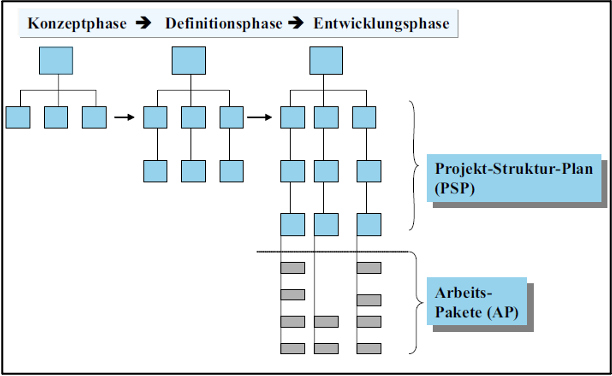
\includegraphics[width=0.47\linewidth]{graphics/psp.png}
%     \caption{Zuordnung von Arbeitspaketen innerhalb der Projektstrukturplanung.}\label{abb:psp}
% \end{figure}
% \section{Arbeitspaketebeschreibung und Aufwandsschätzung}
% Bestandteile bei der Defintion von Arbeitspaketen sind die Leistungsbeschreibung, die jeweils verantwortliche Person
% sowie die zugeordneten Ressourcen.
% \footcite[Vgl.][73]{gadatschGrundkursITProjektcontrollingGrundlagen2008}
% Zusätzlich können untergeordnete Aufgabenpakete mit entsprechenden Zeitangaben erstellt werden.
% \footcite[Vgl.][74]{gadatschGrundkursITProjektcontrollingGrundlagen2008}
% Als Ergebnis muss denoch schlussendlich ein minimal funktionsfähiges Produkt (in der Literatur: „\ac{MVP}“)
% vorliegen, welches im Sinne des Wasserfall-Modells in die nächste Phase übernommen werden kann.
% \footcite[Vgl.][52]{panagosToolsUndMassnahmen2019}
% Als weitere Anforderung an die Arbeitspakete soll beim vorliegenden Projekt dafür gesorgt sein, dass die Ausführung
% von einer einzelnen Person in einem angemessenen zeitlichen Rahmen bewältigt werden kann.
% In Projekten, welche unter wirtschaftlichen Rahmenbedingungen stattfinden, werden für die Schätzung des Zeitbedarfs
% der einzelnen Projektaktivitäten häufig \ac{PM} benutzt, bei welchen allerdings Vollzeitmitarbeiter als Grundlage
% angesehen werden.
% \footcite[Vgl.][74]{gadatschGrundkursITProjektcontrollingGrundlagen2008}
% Da dieser Umstand bei einem Hochschulprojekt nicht gegeben ist, wird daher mit keiner konkret geschätzten Zeit
% gearbeitet. Es wird hier nach interner Absprache zwischen dem Projektteam lediglich eine Abgabefrist für
% Arbeitspakete gesetzt, welche für alle am Projekt beteiligten Personen einzuhalten ist. Weitere Informationen
% hierzu sind in \textit{Kapitel 6} zu finden.
% \section{Backlog und Akzeptanzkriterien für Arbeitspakete}
% Das Backlog stellt eine Liste der gewünschten Arbeiten dar.
% \footcite[Vgl.][362]{kusay-merkleAgilesProjektmanagementIm2018}
% Diese noch zu erledigenden Aufgaben können dort bis zur abschließenden Nutzung gesammelt und aufbereitet werden.
% \footcite[Vgl.][362]{kusay-merkleAgilesProjektmanagementIm2018}
% Ferner werden die Arbeitspakete hierbei den großen Meilensteinen (in der Literatur: „Epics“) zugeordnet.
% Als Werkzeug für diese Arbeitspakete- und Zeitplanung kommt das Programm „Jira Software“ zum Einsatz.
% Es ist für kleine Projekte kostenlos nutzbar und enthält Funktionen für die Nachvollziehbarkeit von Aufgaben
% und Fehlern sowie für die Verwaltung von Projekten.
% \footcite[Vgl.][3]{ortuMeasuringUnderstandingEffectiveness2015}
% Als vorteilhaft bei der Nutzung von Jira erweist sich der grundflexible Charakter der Software, welcher
% es dem Projektteam unter anderem ermöglicht, Teilinkremente mit hoher Produktivität auszuliefern, das Backlog zu verwalten
% sowie den Fortschritt des Projekts visuell darzustellen.
% \footcite[Vgl.][3]{ortuMeasuringUnderstandingEffectiveness2015}
% Die aktuellen Meilensteine im Backlog sind folgende:
% \begin{enumerate}
%     \item Ausarbeitung der Projektkonzeption
%     \item Präsentation am Anfang des sechsten Semesters
%     \item Interviews mit Leitfaden
%     \item Wissenschaftliche Ausarbeitung im sechsten Semester
%     \item Prototyp im sechsten Semester
%     \item Ergebnispräsentation am Ende des sechsten Semesters
% \end{enumerate}
% Im Backlog werden schließlich für die einzelnen Arbeitspakete der Meilensteine Kriterien erstellt, anhand derer
% erkenntlich wird, ob das jeweilige Objekt den Anforderungen entsprechend umgesetzt worden ist.
% \footcite[Vgl.][46]{kusay-merkleAgilesProjektmanagementIm2018}
% Vor der Fertigstellung eines Arbeitspakets müssen alle vorher definierten Akzeptanzkriterien erfüllt sein.
% \footcite[Vgl.][154]{kusterHandbuchProjektmanagementAgil2022}
\chapter{Technische Umsetzung}
\section{Anforderungen und Rahmenbedingungen}
Als Anforderungen und Rahmenbedingungen für die technische Umsetzung des Projektes
werden die folgenden Punkte festgelegt:
\section{Programmatische Konfiguration in Moodle}
\section{Gestaltung der Zertifizierung}
David


% In Unternehmen werden Schnittstellen zwischen verschiedenen Projekten durch den Einsatz eines Projektportfolio-Managements überwacht und dirigiert.
% \footcite[Vgl.][S. 356 f.]{bilginHandlingProjectDependencies2017}
% Die Einflüsse der anderen Projekte werden offensichtlich, wenn die Abhängigkeiten, welche durch die Aufgabengebiete definiert sind,
% dargestellt werden. Diese Einflüsse können, wie im Kapitel Risiko erläutert, überaus Einfluss auf die Qualität und die Zeitplanung des Projektes haben.
% Um diesen Einfluss darstellen zu können, wird die Kontextebene des C4-Modells verwendet, um einen Überblick über die Schnittstellen zu erhalten.
% \begin{figure}[H]
%     \centering
%     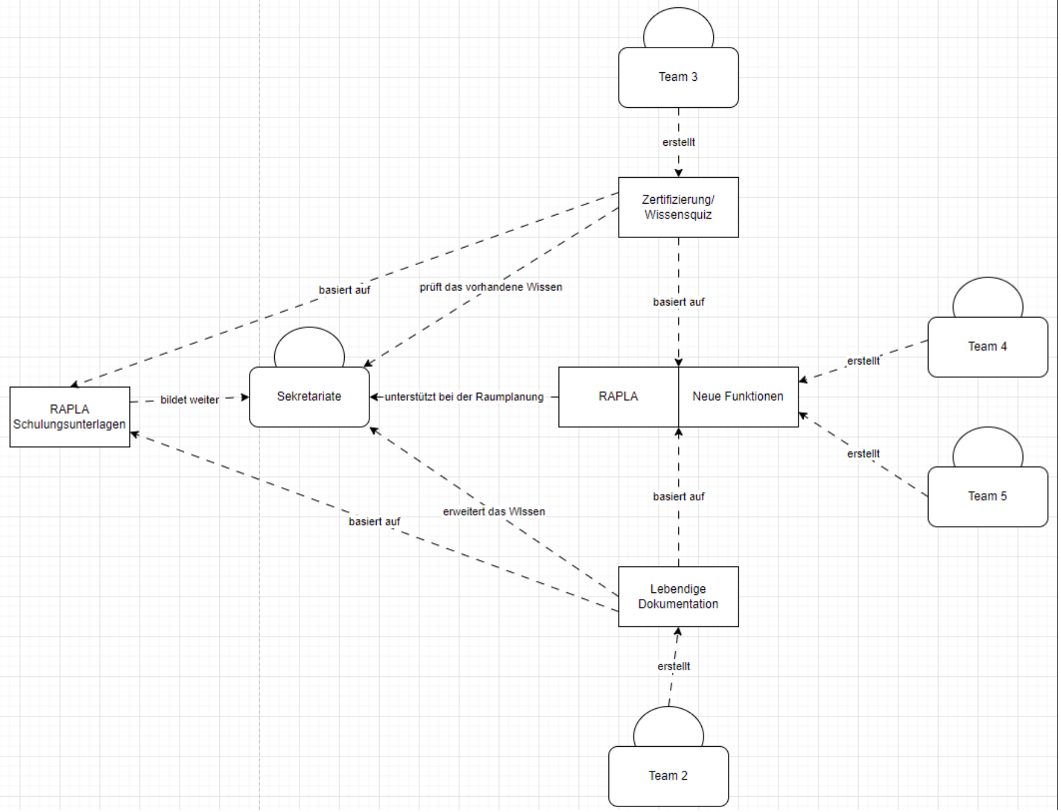
\includegraphics[width=1\linewidth]{graphics/rapla_model.png}
%     \caption{Schnittstellen im vorliegenden Projekt.}\label{abb:zeitplanung}
% \end{figure}
% Wie an diesem Modell sichtbar, gibt es für dieses Projekt (Team drei) 
% hauptsächlich eine direkte Abhängigkeit zu den Teams vier und fünf, da die
% Zertifizierung bestenfalls neue Funktionen von \ac{RAPLA} berücksichtigt und prüft. Allerdings
% gibt es auch eine indirekte Schnittstelle zu Team zwei, da diese ihre lebendige Dokumentation
% auf den gleichen Quellen (\ac{RAPLA} und \ac{RAPLA} Schulungsunterlagen) aufbaut. Durch klare Absprache
% können Mehrarbeit und Dopplungen vermieden werden.

% Aufbauend auf diesen Schnittstellen wird für die Zukunft folgende Zusammenarbeits-Maxime definiert: 
% Die Entwicklung der Teams vier und fünf werden verfolgt und es werden bereits vor deren Fertigstellung Platzhalter
% in der Zertifizierung geschaffen, um die Entwicklungen direkt nach ihrer Fertigstellung gegebenenfalls in die
% Zertifizierung aufnehmen zu können (soweit sie auch von den Schulungsunterlagen aufgenommen werden).
% Während sich die Interaktion mit den Teams Teams vier und fünf eher auf die zweite Hälfte des Projektes
% beziehen wird, besteht das Absprache-Potenzial mit Team zwei von Beginn an. Daher werden regelmäßige Absprachen
% sowie ein Austausch von Informationen geplant. Zusätzlich werden außerplanmäßige Treffen bei der Koordination
% von bestimmten Arbeitspaketen oder zu besonderen Anlässen wie Rücksprachen mit den Stakeholdern stattfinden.
\chapter{Erprobung und Evaluation}
\section{Erprobung durch die Zielgruppe}
\section{Analyse der Erprobungsresultate}
\section{Ableitung von Optimierungsmaßnahmen}
David
% Die Zeitplanung spielt im Kontext des Hochschulprojektes eine bedeutende Rolle,
% da das Projekt zeitlich eng begrenzt und auf zwei verschiedene Semester aufgeteilt ist.
% Es ergibt sich die Notwendigkeit einer detaillierten Planung, um alle Anforderungen
% termingerecht erfüllen zu können und Abhängigkeiten zwischen mehreren Teammitgliedern
% konfliktfrei zu lösen. Weiterhin müssen separate Planungen für die jeweiligen Semester
% durchgeführt werden, da diese zwar abhängig voneinander sind, die Informationen für die
% Planung des höheren Semesters allerdings noch nicht vorhanden sein müssen.

% Die Planung dazu basiert - wie in vorherigen Kapiteln beschrieben - allgemein auf
% festen Abgabeterminen zu bereits festgelegten Meetings. 
% Begonnen wurde mit der groben Definition von Epics
% und Arbeitspakten in Jira, auf deren Basis dann eine vorläufige Planung für beide Semester
% erstellt wurde. Diese konnte schrittweise in ihrem Detailgrad ausgebaut werden.

% Zur Visualisierung wurde die Zeitleiste in Jira verwendet, die einem Gantt-Diagramm ähnelt.
% Das Gantt-Diagramm bietet sich bei der Zeitplanung hierbei besonders an, da es eine
% übersichtliche Möglichkeit bietet, Verknüpfungen mit vorangehenden Vorgängen,
% Dokumentation der Vorgangsverantwortlichen sowie Kapazitätsdarstellungen, in einem
% Diagramm zu veranschaulichen.
% \footcite[Vgl.][123]{osterhageAnhangProjektmanagement2016}
% Dadurch, dass über die Zeitachse Aktivitäten in Form von Balken mit festen Anfangs-
% und Endtermin dargestellt werden, können Abhängigkeiten zwischen Aufgaben und
% Arbeitspaketen hergestellt sowie kritische Stellen in der Planung sichtbar gemacht
% werden.
% \footcite[Vgl.][117]{hobelGABLERBUSINESSWISSENAZ2006}
% Zudem erklärt sich die populäre Nutzung von Gantt-Charts auch dadurch, dass
% sie sowohl den Projektteilnehmern eine übersichtliche Visualisierung des Projektfortschritts
% ermöglichen als auch in der finalen Präsentation der Ergebnisse vor dem Management genutzt
% werden können.
% \footcite[Vgl.][435]{wilsonGanttChartsCentenary2003}
% \begin{figure}[H]
%     \centering
%     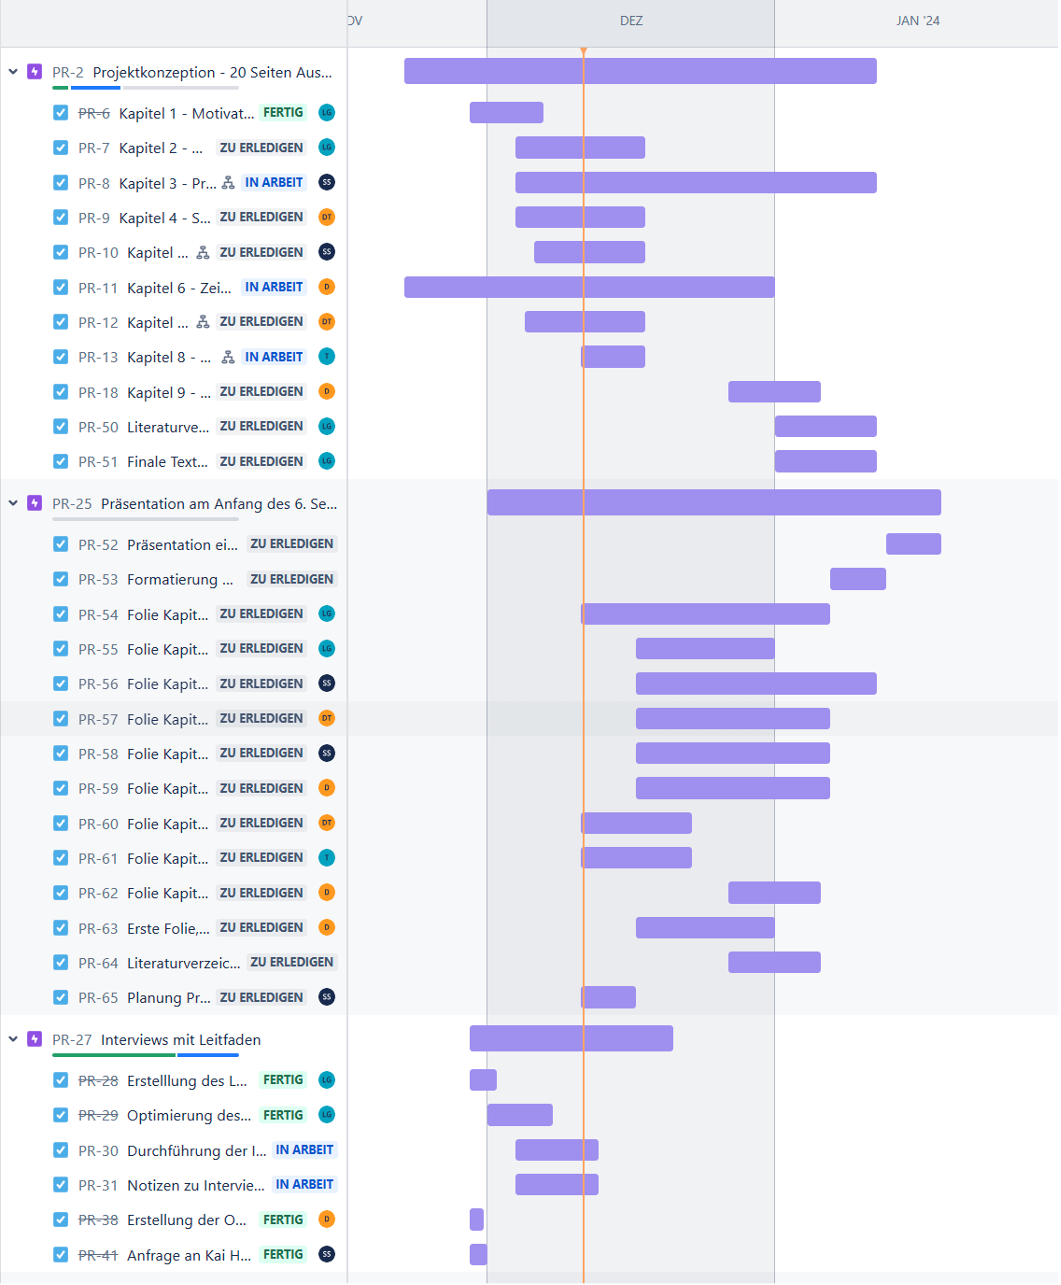
\includegraphics[width=0.9\linewidth]{graphics/zeitplanung.png}
%     \caption{Übersicht über die Zeitplanung in JIRA.}\label{abb:zeitplanung}
% \end{figure}
% Es wird sichtbar, dass die Kapitel nach einer logischen Reihenfolge eingeteilt worden sind.
% Allgemeine Planungsthemen wie Projektplanung oder
% Zeitplanung sind auf einen größeren Zeitraum zugeschnitten, konkrete Kapitelthemen wie die
% Einleitung oder auch die Anforderungen dagegen für kurze und spezifische Zeitperioden vorgesehen
% sowie in einer für den Ablauf effizienten, sequenziellen Reihenfolge angeordnet. Hieraus ergibt
% sich, dass das sechste Semester überwiegend für die Umsetzung genutzt werden kann und jegliche
% Planung bereits zu großen Teilen finalisiert ist.

% Bezüglich der Umsetzungsplanung lässt sich feststellen, dass die Umsetzung der Schulungsunterlage
% einige Abhängigkeiten mit sich bringt. So erfordert sie enge Absprachen mit dem zweiten
% Schulungs-Team, um keine Dopplungen zu erhalten. Diese Planung kann sich jedoch aufgrund
% des neuen Vorlesungsplans im sechsten Semester noch ändern. 


\chapter{Ergebnisdiskussion}
\section{Auftrag des Projektes}
\section{Kritische Reflexion der Ergebnisse}
\section{Implikationen für Theorie und Praxis}
\section{Ausblick}
Bevor eine Analyse der Risiken durchgeführt werden kann, müssen zunächst die Terminologie und die Ziele der Durchführung näher dargelegt werden. 
Für die Definition des Risikos wird die engere Definition des Risikos aus dem Fachbuch „IT-Risikomanagement mit System“ von Hans-Peter Königs verwendet. 
Die engere Definition des Risikos umfasst eine Abweichung von einem vorher definierten Ziel.
\footcite[Vgl.][12]{koenigsITRisikomanagementMitSystem2017}
Bei einem Projekt ist das Ziel der erfolgreiche Abschluss des Projekts.
Gegenübergestellt kann es Abweichungen in Dauer, Budget und Qualität geben, die den Erfolg des Projekts negativ beeinflussen.
\footcite[Vgl.][13]{koenigsITRisikomanagementMitSystem2017}
Die Evidenz für die kritische Relevanz der Risikoabschätzung im Projektkontext führt zu einer großen
Menge an wissenschaftlichen und unternehmerischen Quellen, die sich mit dem Risiko-Management beschäftigen.
Das Versagen der Verantwortlichen im Umgang mit Risiken führt zu zahlreichen Möglichkeiten für kontraproduktive Ausgänge für das Projekt und im schlimmsten Fall für das Projektumfeld.
Ein Beispiel für das Scheitern der Handhabung von Risiken lässt sich im Finanzbereich finden.
Dort arbeiteten viele Akteure wiederkehrend nicht anforderungskonform, was schließlich in der Finanzkriese 2008 resutlierte.
\footcite[Vgl.][39]{stulzRiskManagementFailures2008}
Die hauptsächlichen Fehler, die sich als kritisch erwiesen haben, sind die Fehleinschätzung von Risiken,
vernachlässigte, ignorierte oder unbekannte Risiken, fehlende Kommunikation und Intransparenz in der Darstellung und Steuerung von Risiken.
\footcite[Vgl.][S. 42 ff.]{stulzRiskManagementFailures2008}
Damit diese Fehler vermindert auftreten, beschäftigen sich wissenschaftliche Quellen mit dem Management von Risiken,
um in der Praxis Möglichkeiten für Bewerkstellligung von Kalkulation, Prognose und mögliche Interventionen umsetzen zu können.
In der Projektkonzeption und der Einleitung zur Risikoplanung ist es daher essenziell, diese Erkenntnisse zu berücksichtigen
und ein umfassendes Risikomanagement zu implementieren. Dabei kann ein Projekt in sechs Risikomanagement-Phasen kontinuierlich begleitet werden.
\footcite[Vgl.][45]{dikmenLearningRisksTool2008}
In der ersten Phase werden Risiken identifiziert, indem Risikoinformationen und Unsicherheiten zusammengetragen und dokumentiert werden.
In der zweiten Phase wird eine Bewertung der Risiken durchgeführt, um diese in der dritten Phase angemessen handhaben zu können.
Diese ersten drei Phasen können innerhalb der Projektkonzeption bereits durchgeführt werden.
Während der Projektdurchführung werden iterativ die Phasen vier und fünf durchgeführt. Die vierte
Phase beschäftigt sich mit der Überwachung von Risiken und die fünfte Phase mit den Interventionen im
Umgang mit Risiken, falls diese eintreten oder sich die Einschätzung ändert. Am Ende eines Projekts
sollte in einer letzten Phase eine Evaluation des Risikomanagements stattfinden.

Ergänzend zu diesen Phasen des Risikomanagements existieren Maßnahmen, um auf die einzelnen Risiken zu reagieren.
\footcite[Vgl.][S. 22 f.]{brandstaeterAgileITProjekteErfolgreich2013}
Diese Maßnahmen lassen sich aufschlüsseln in Maßnahmen, die präventiver Natur sind, sowie in solche, die erst beim Eintreten
eines Risikos ausgelöst werden, um die Risikoauswirkungen einzudämmen.
Ein Beispiel für den Unterschied dieser Maßnahmen ist der Umgang mit Bränden in Gebäuden.
In vielen Gebäuden ist das Rauchen und Erzeugen eines offenen Feuers verboten, um präventiv zu verhindern, dass ein Brand ausbricht.
Allerdings werden zur Bekämpfung eines Feuers zusätzlich Feuerlöscher für den Fall bereitgestellt, dass ein Brand ausbrechen sollte.
Eine Unterscheidung dieser Maßnahmentypen für eine Risikoanalyse kann Mehrwert schaffen, um die reale Gefahr darstellen zu können.
In der ersten Risikomanagementphase (Risikoidentifikationsphase) werden die Hauptrisiken des Scrum-Verfahrens
als Leitrisikotypen verwendet\footcite[Vgl.][40]{brandstaeterAgileITProjekteErfolgreich2013}: 
Anhand dieser Hauptrisiken werden potenzielle Probleme und Herausforderungen für das bestehende Projekt abgeleitet.
Ebenso werden zur Vermeidung und Bewerkstelligung von Risiken präventive und reaktive Maßnahmen erarbeitet, welchen
als Leitbild ein entsprechendes Risikoregister zugrunde liegt.


\chapter*{Anhang}
\addcontentsline{toc}{chapter}{Anhang}
\section*{Anhangverzeichnis}
\vspace{-8em}

% vor \listofanhang müssen Einrückungen angepasst werden
\abstaendeanhangverzeichnis

\listofanhang
\clearpage
\spezialkopfzeile{Anhang} % damit in der Kopfzeile das Wort "Anhang" angezeigt wird

\anhang{Projektrollen und Verantwortlichkeiten}\label{anhang:kap1}
% \anhangteil{Unterkapitel 1}\label{anhang:ukap1}
\begin{figure}[H]
  \centering
  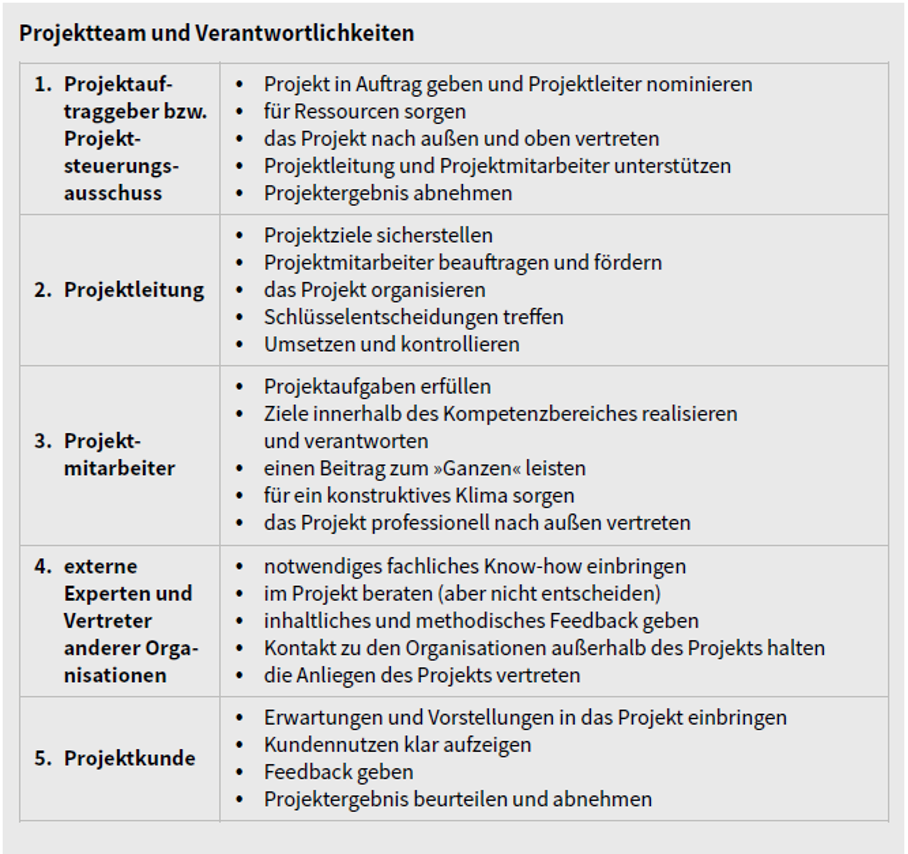
\includegraphics[width=0.8\linewidth]{graphics/pr_ve.png}
  \caption[Rollen und Verantwortlichkeiten in Projekten.]{Rollen und Verantwortlichkeiten in Projekten.\protect\footnotemark}\label{abb:pr_ve}
\end{figure}
\footnotetext{\cite[Enthalten in:][90]{stoegerWirksamesProjektmanagementMit2019}}
\anhang{Discord-Server Organisationsstruktur}\label{anhang:kap2}
\anhang{Risikomatrix}\label{anhang:kap3}


\lstset{language=TeX, % hervorzuhebende Keywords definieren
  morekeywords={anhang, anhangteil}
}

% \blinddocument
% \chapter{Beispiele für Abbildungen und Tabellen}\label{chapter:abbildungenTabellen}

Hier finden Sie Beispiele für Abbildungen, Tabellen, Formelsatz und  Source Code.

\section{Abbildungen}
In diesem Abschnitt gibt die Abbildungen~\ref{abb:Logo2cmHoch} und~\ref{abb:Logo2cmBreit}, die beide das Logo der DHBW zeigen.

\begin{figure}[htb]
\centering

\includegraphics[height=2cm]{graphics/dhbw.png}
\caption[DHBW-Logo 2cm hoch]{DHBW-Logo 2cm hoch.\footnotemark}
\label{abb:Logo2cmHoch}
\end{figure}
\footnotetext{Mit Änderungen entnommen aus: \cite{OhneAutorenOhneJahr}}

\lstset{language=TeX, % hervorzuhebende Keywords definieren
  morekeywords={footnotetext,footnotemark,footcite,caption}
}

\emph{Spezialfall:} Sofern \emph{innerhalb} der Bezeichnung einer Abbildung eine Fußnote angegeben oder eine Quelle referenziert werden soll, geschieht dies nicht per \lstinline|\footnote| oder \lstinline
|\footcite|. Vielmehr sind die Befehle \lstinline|\footnotemark| und \lstinline|\footnotetext| zu verwenden und außerdem das optionale Argument für \lstinline|\caption| anzugeben (vgl.\ Source Code).

\begin{figure}[htb]
\centering

\includegraphics[width=2cm]{graphics/dhbw.png}
\caption[DHBW-Logo 2cm breit.]{DHBW-Logo 2cm breit. (Quelle: DHBW\footnotemark)}
\label{abb:Logo2cmBreit}
\end{figure}
\footnotetext{\url{www.dhbw.de}}



\section{Tabellen}

In diesem Abschnitt gibt es zwei Beispiel-Tabellen, nämlich auf Seite~\pageref{tab:BeispielTabelleKlein} und auf Seite~\pageref{tab:BeispielTabelleGroesser}.

\begin{table}[htb]
\centering
\begin{tabular}{lcr}
links & Mitte & rechts \\
\hline
Muster & Muster & Muster \\
\end{tabular}
\caption{Kleine Beispiel-Tabelle.}
\label{tab:BeispielTabelleKlein}
\end{table}

\begin{table}[htb]
\centering
\begin{tabular}{|l|l|c|l|r||l}
    \textbf{Spalte 1} & \textbf{Spalte 2} & \textbf{Spalte 3} & \textbf{Spalte 4} & \textbf{Spalte 5} & \textbf{Spalte 6} \\
    \hline
    a        & b          & c                & d        & e        & f        \\
    Test     & Test, Test & Test, Test, Test & ~        & ~        & ~        \\
    1        & 2          & 3                & 4        & 5        & 6        \\
\end{tabular}
\caption{Größere Beispiel-Tabelle.}
\label{tab:BeispielTabelleGroesser}
\end{table}

\section{Etwas Mathematik}

Eine abgesetzte Formel:
\[
  \int_a^b x^2 \: \mathrm{d} x = \frac{1}{3} (b^3 - a^3)
\]

Es ist $a^2+b^2 = c^2$ eine Formel im Text.

\section{Source Code}

Source Code-Blöcke können auf folgende Arten eingefügt werden:

\lstset{language=Java}

Direkt im \LaTeX-Source Code:
\begin{lstlisting}
if(1 > 0) {
  System.out.println("OK"); 
} else {
  System.out.println("merkwuerdig");
}
\end{lstlisting}

oder eingefügt aus einer externen Datei.
\lstinputlisting{includes/HelloWorld.java}

% \anhang{Release Notes}
\anhangteil{Änderungen in Version 1.1}\label{anhang:ReleaseNotes11}
In Version 1.1 sind einige Rückmeldungen, die nach der Einführungsvorlesung am 6.2.2015 oder nach Veröffentlichung der Vorlage in Moodle eingegangen sind, berücksichtigt worden. Korrekturen sind mit \enquote{(Fix)} gekennzeichnet. 

\begin{itemize}
\item \verb|latex-vorlage.tex|
\begin{itemize}
\item (Fix) Abkürzungsverzeichnis wird vor Abbildungsverzeichnis platziert
\item (Fix) Abbildungs- und Tabellenverzeichnis in Inhaltsverzeichnis aufgenommen
\item (Fix) Quellenverzeichnis wird nun ohne Kapitelnummer dargestellt

\item eingebundene Dateien in Unterverzeichnissen \verb|includes| bzw.\ \verb|graphics|
\item Beispiel-Anhang (Datei \verb|anhang.tex|) mit Erklärungen wurde eingebunden 
\end{itemize}

\item \verb|_dhbw_praeambel.tex|
\begin{itemize}
\item (Fix) das Paket hyperref wird nach biblatex eingebunden, um ein Problem mit der Verlinkung der Fußnoten im PDF zu beheben
\item (Fix) Fußnoten  gemäß der Richtlinien fortlaufend nummeriert und nicht pro Kapitel
\item Einstellungen hinzugefügt, um Anhangsverzeichnis zu ermöglichen
\item bessere Kompatibilität zwischen KOMA-Script (scrreprt) und anderen Paketen mittels scrhack
\end{itemize}

\item \verb|_dhbw_biblatex-config.tex|
\begin{itemize}
\item (Fix) keine Abschnittsnummern für einzelne Verzeichnisse im Quellenverzeichnis
\end{itemize}

\item \verb|abbildungen_und_tabellen.tex|
\begin{itemize}
\item Erklärung, wie eine Fußnote/ein Zitat bei einer Abbildung zu erstellen ist
\end{itemize}

\item \verb|abkuerzungen.tex|
\begin{itemize}
\item Abkürzungsverzeichnis wird im Inhaltsverzeichnis aufgeführt
\end{itemize}

\item \verb|abstract.tex|, \verb|anhang.tex|, \verb|einleitung.tex| 
\begin{itemize}
\item Erklärungen im Text ergänzt
\end{itemize}

\item \verb|deckblatt.tex|
\begin{itemize}
\item Meta-Daten (Autor, Titel) für die generierte PDF-Datei lassen sich nun festlegen
\end{itemize}

\end{itemize}


\anhangteil{Änderungen in Version 1.2}\label{anhang:ReleaseNotes12}
Über das Forum in Moodle sind einige Rückmeldungen eingegangen -- vielen Dank an alle, die dazu beigetragen haben. In der Version 1.2 wurden folgende Änderungen vorgenommen, wobei Korrekturen wieder mit \enquote{(Fix)} gekennzeichnet sind: 

\begin{itemize}
\item \verb|latex-vorlage.tex| (Hauptdokument)
\begin{itemize}
\item (Fix) Zeile 19: Seitenzahlen zu Beginn mit römischen \emph{Groß}buchstaben nummeriert
\end{itemize}

\item \verb|_dhbw_praeambel.tex|
\begin{itemize}
\item Zeile 39/40: Unterstützung für \enquote{ebenda} 
\item Zeile 46--68: zweite Gliederungsebene für Anhänge ermöglicht
\item (Fix) Zeile 70--73: Abbildungen und Tabellen: Zähler fortlaufend, kein Rücksetzen zu Kapitelbeginn (Paket \verb|chngcntr| anstelle von Paket \verb|remreset|)
\end{itemize}

\item \verb|_dhbw_biblatex-config.tex|
\begin{itemize}
\item (Fix) bei Quellen mit Herausgeber, aber ohne Autor wird der Name des Herausgebers im Verzeichnis fett gedruckt
\item Unterstützung für \enquote{ebenda} 
\end{itemize}

\item \verb|abkuerzungen.tex|
\begin{itemize}
\item Bemerkungen zur fortgeschrittenen Nutzung des \verb|acronym|-Pakets eingefügt 
\end{itemize}

\item \verb|einleitung.tex|
\begin{itemize}
\item Abschnitt 1.3 zu Einstellungen ergänzt
\item Abschnitt 1.5 zu Fehlerbehebungen eingefügt 
\end{itemize}

\item \verb|text-mit-zitaten.tex|
\begin{itemize}
\item Abschnitt 3.1 eingefügt, Erläuterungen zum Zitieren mit \enquote{vgl.} und \enquote{ebenda}. 
\item Abschnitt 3.2: Beispiele ergänzt
\item Hinweis zu Jahreszahlen bei Online-Quellen
\end{itemize}

\item \verb|anhang.tex|
\begin{itemize}
\item Erläuterungen zur zweiten Gliederungsebene
\end{itemize}

\item \verb|literatur-datenbank.bib|
\begin{itemize}
\item weitere Beispiele für Quellen
\end{itemize}

\end{itemize}

\anhangteil{Änderungen in Version 1.3}\label{anhang:ReleaseNotes13}
Durch die ab 1/2016 geltenden Änderungen der Zitierrichtlinien des Studiengangs waren einige kleinere Anpassungen der Vorlage erforderlich, die nachfolgend beschrieben sind. Bei dieser Gelegenheit ebenfalls erfolgte Korrekturen sind wieder mit \enquote{(Fix)} gekennzeichnet:

\begin{itemize}
\item \verb|latex-vorlage.tex| (Hauptdokument)
\begin{itemize}
\item Hinweis auf Option doppelseitiger Druck entfernt
\item Schriftgröße der Kapitelüberschriften verkleinert
\item (Fix) Kopf- und Fußzeilen werden nun korrekt angezeigt für erste Seite eines Kapitels und auch  Quellenverzeichnisse
\end{itemize}

\item \verb|_dhbw_praeambel.tex|
\begin{itemize}
\item Angabe des unteren Rands für Seitenzahl, da diese nun unten rechts steht
\item Unterstützung für \enquote{ebenda} entfernt
\item (Fix) Präfixe wie \enquote{von} im Namen eines Autors werden berücksichtigt
\item Anpassung der Abstände bei Kapitelüberschriften
\item Kopf- und Fußzeile für Verzeichnisse nun in \verb|_dhbw_kopfzeilen.tex| definiert 
\end{itemize}


\item \verb|deckblatt.tex|
\begin{itemize}
\item Schriftgröße des Titels vergrößert
\item Befehl \verb|\typMeinerArbeit| eingeführt, um Typ auszuwählen
\item Festlegung des Themas (für ehrenwörtliche Erklärung) mit Befehl \verb|\themaMeinerArbeit|
\item Darstellung der Angabe des Betreuers in der Ausbildungsstätte angepasst
\item Formulierung des Sperrvermerks angepasst  
\end{itemize}

\item \verb|_dhbw_erklaerung.tex|
\begin{itemize}
\item Formulierung angepasst an geänderte Prüfungsordnung
\item Typ und Thema der Arbeit werden automatisch eingefügt
\end{itemize}

\item \verb|_dhbw_kopfzeilen.tex|
\begin{itemize}
\item Seitennummern stehen jetzt unten rechts
\item (Fix) Kopf- und Fußzeile werden nun korrekt angezeigt in Verzeichnissen und dem Anhang
\end{itemize}

\item \verb|_dhbw_biblatex-config.tex|
\begin{itemize}
\item Anpassung des Zitierstils auf die ab 1/2016 geltenden Regelungen  
\item Vorkehrungen für Eindeutigkeit (Hinzufügen abgekürzter oder nötigenfalls ausgeschriebener Vorname) bei Übereinstimmung von Name und Jahreszahl 
\end{itemize}

\item \verb|einleitung.tex|
\begin{itemize}
\item Abschnitt 1.3 zu Einstellungen grundlegend überarbeitet
\item Abschnitt 1.5.2 zur Kontrolle der Seitenränder eingefügt 
\end{itemize}

\item \verb|text-mit-zitaten.tex|
\begin{itemize}
\item Abschnitt 3.1: Hinweise zu \enquote{ebenda} entfernt
\item Abschnitt 3.2: Beispiele zur Eindeutigkeit des Zitats ergänzt
\item Abschnitt 3.3: Hinweise für E-Journals/E-Books ergänzt 
\end{itemize}

\item \verb|anhang.tex|
\begin{itemize}
\item (Fix) Befehl \verb|\spezialkopfzeile| aufgenommen, damit in Kopfzeile das Wort \enquote{Anhang} angezeigt wird 
\item diese Release Notes wurden in eine eigene Datei verschoben
\end{itemize}

\item \verb|release_notes.tex|
\begin{itemize}
\item s.o.
\end{itemize}


\item \verb|literatur-datenbank.bib|
\begin{itemize}
\item weitere Beispiele für Quellen
\end{itemize}
\end{itemize}

\anhangteil{Änderungen in Version 1.4}\label{anhang:ReleaseNotes14}
Durch nicht abwärtskompatible Änderungen beim Versionswechsel von Biblatex 3.2 zu 3.3 sind einige Änderungen notwendig geworden.\footnote{Diese basieren auf Vorschlägen von Yannik Ehlert -- vielen Dank dafür!}
Die vorliegende Version 1.4 wurde erfolgreich mit MikTeX gestestet (portable Version 2.9.6361 vom 3.6.2017, unter Verwendung von Biblatex 3.7).

\begin{itemize}
\item \verb|_dhbw_biblatex-config.tex|
\begin{itemize}
\item Anpassung der \verb|\usebibmacro|-Befehle
\end{itemize}

\item \verb|_dhbw_authoryear.bbx|
\begin{itemize}
\item  Änderung von \verb|\printdateextralabel| zu \verb|\printlabeldateextra|
\end{itemize}
\end{itemize}

\anhangteil{Änderungen in Version 1.5}\label{anhang:ReleaseNotes15}
Für den Test dieser Version auf einem Windows-System wurde wieder die portable Version von MiKTeX (2.9.6521 vom 10.11.2017) verwendet.\footnote{\url{http://miktex.org/portable}} Da in diesem Paket leider die Versionen von Biblatex (3.10) und Biber (2.7) inkompatibel sind, ist es erforderlich, die Datei \verb|biber.exe| im Verzeichnis \verb|texmfs\install\miktex\bin\| durch die aktuelle Version 2.10 vom 20.12.2017\footnote{\url{https://sourceforge.net/projects/biblatex-biber/files/biblatex-biber/current/binaries/Windows/}} zu ersetzen. Im Editor TeXworks verwendet man dann zum Übersetzen des \LaTeX-Sourcecodes Typeset/pdfLaTeX bzw.\ Typeset/Biber.

Korrekturen sind wieder mit \enquote{(Fix)} gekennzeichnet.

\begin{itemize}
\item \verb|latex-vorlage.tex| (Hauptdokument)
\begin{itemize}
\item Nach der Änderung der Zitierrichtlinien gibt es nun kein separates Verzeichnis mehr für Internet- und Intranetquellen.
\item Option \verb|notkeyword=ausblenden| bei \verb|\printbibligraphy| sorgt dafür, dass Sekundärliteratur korrekt zitiert wird.
\end{itemize}

\item \verb|_dhbw_praembel.tex|
\begin{itemize}
\item (Fix) Die Bezeichnung geschachtelter Anhänge wurde auf das in den Zitierrichtlinien geforderte Format \enquote{Anhang 2/1} angepasst (Befehl \verb|\anhangteil|).
\end{itemize}

\item \verb|einleitung.tex|
\begin{itemize}
\item Hinweis zum Ausblenden der farbigen Links im PDF hinzugefügt
\end{itemize}

\item \verb|text-mit-zitaten.tex|
\begin{itemize}
\item Abschnitt 3.4 aktualisiert nach Wegfall des separaten Verzeichnisses für Internet- und Intranetquellen
\item Abschnitt zum Zitieren von Sekundärliteratur hinzugefügt
\end{itemize}

\end{itemize}


\anhangteil{Änderungen in Version 1.6}\label{anhang:ReleaseNotes16}
Diese Version wurde auf einem Windows-System erfolgreich mit der portablen Version von MiKTeX (2.9.6621 vom 18.02.2018) getestet.\footnote{Vielen Dank an Florian Eichin für seine wertvollen Anmerkungen.}

Korrekturen sind wieder mit \enquote{(Fix)} gekennzeichnet.

\newpage

\begin{itemize}
\item \verb|latex-vorlage.tex| (Hauptdokument)
\begin{itemize}
\item (Fix) An einer Stelle gab es in Version 1.5 (Internetquellen nicht mehr separat) noch ein Überbleibsel von Version 1.4 (Internetquellen separat), dies wurde korrigiert.
\item (Fix) Im Inhaltsverzeichnis war die Verlinkung des Abbildungs- und Tabellenverzeich\-nisses nicht ganz korrekt.
\item Mit den Befehlen \verb|\literaturverzeichnis| bzw.\ \verb|\literaturUndQuellenverzeichnis| kann bequem die Erstellung der Quellenverzeichnisse gesteuert werden, abhängig davon, ob es ein Gesprächsverzeichnis gibt oder nicht.
 
\end{itemize}

\item \verb|_dhbw_praembel.tex|
\begin{itemize}
\item Einrückungen für Abbildungs-, Tabellen- und Anhangverzeichnis angepasst
\item Abkürzungen \enquote{Abb.} und \enquote{Tab.} für Abbildungen bzw.\ Tabellen
\end{itemize}

\item \verb|_dhbw_biblatex-config.tex|
\begin{itemize}
\item Befehle \verb|\literaturverzeichnis| und \verb|\literaturUndGespraechsverzeichnis| definiert
\item Befehl \verb|\footcitePrimaerSekundaer| definiert
\end{itemize}

\item \verb|_dhbw_erklaerung.tex|
\begin{itemize}
\item Eintrag als \enquote{Erklärung} (statt \enquote{Ehrenwörtliche Erklärung}) ins Inhaltsverzeichnis
\end{itemize}

\item \verb|einleitung.tex|
\begin{itemize}
\item Bezeichnung \enquote{Erklärung} statt \enquote{Ehrenwörtliche Erklärung}
\item Erläuterung von \verb|\literaturverzeichnis| und \verb|\literaturUndGespraechsverzeichnis|
\item Hinweis auf Notwendigkeit von Updates bei MikTeX Portable
\end{itemize}

\item \verb|text_mit_zitaten.tex|
\begin{itemize}
\item Erläuterungen zu Befehl \verb|\footcitePrimaerSekundaer| ergänzt
\end{itemize}

\item \verb|anhang.tex|
\begin{itemize}
\item Befehl \verb|\abstaendeanhangverzeichnis| für Anpassung Einrückung ergänzt
\end{itemize}

\item \verb|literatur-datenbank.bib|
\begin{itemize}
\item Eintrag ergänzt
\end{itemize}

\end{itemize}

\anhangteil{Änderungen in Version 1.7}\label{anhang:ReleaseNotes17}
Diese Version wurde auf einem Windows-System erfolgreich mit der portablen Version von MiKTeX (2.9.6942 vom 04.01.2019) getestet.

Korrekturen sind wieder mit \enquote{(Fix)} gekennzeichnet.

\begin{itemize}
\item \verb|_dhbw-authoryear.bbx|
\begin{itemize}
\item Da \verb|labeldate| in Biblatex nicht mehr unterstützt wird, erfolgte eine Umbenennung in 
\verb|labeldateparts|.\footnote{vgl.\ \url{https://github.com/semprag/biblatex-sp-unified/issues/23}}
\end{itemize}

\item \verb|_dhbw_biblatex-config.tex|
\begin{itemize}
\item (Fix) Es wurde das Problem behoben, dass im Literaturverzeichnis bei bestimmten Eintragstypen der Titel in Anführungszeichen steht.\footnote{Danke an Florian Eichin für seinen Hinweis.}
\end{itemize}

\end{itemize}


\anhangteil{Änderungen in Version 1.8}\label{anhang:ReleaseNotes18}
Diese Version wurde auf einem Windows-System erfolgreich mit der portablen Version von MiKTeX (2.9.6942 vom 04.01.2019) getestet.

Die Aktualisierungen in der Vorlage spiegeln zum Einen die Änderungen in den Zitierrichtlinien wieder. Zum Anderen wurden einige studentische Vorschläge aufgegriffen, um die Nutzung der Vorlage zu erleichtern.\footnote{Danke an Bjarne Koll, Tobias Schwarz und Lars Ungerathen für ihre Anregungen.} 

\begin{itemize}

\item \verb|latex_vorlage.tex| (Hauptdokument)
\begin{itemize}
\item Es wird nun davon ausgegangen, dass die zur Vorlage gehörenden Dateien in einem eigenen Verzeichnis (\verb|template|) liegen.
\item Stellenweise wurden Erläuterungen als Kommentare hinzugefügt.
\end{itemize}

\item \verb|_dhbw_biblatex-config.tex|
\begin{itemize}
\item Code, der mehrere Quellenverzeichnisse unterstützt, wurde entfernt.
\item Ein zu großer Abstand nach Zitaten von Sekundärliteratur wurde korrigiert. 
\end{itemize}

\item \verb|_dhbw_erklaerung.tex|
\begin{itemize}
\item Gemäß der Anforderung in den Zitierrichtlinien wird die Erklärung nicht ins Inhaltsverzeichnis aufgenommen und nicht mit einer Seitenzahl versehen. 
\end{itemize}

\pagebreak
\item \verb|_dhbw_praeambel.tex|
\begin{itemize}
\item Gemäß der Anforderung in den Zitierrichtlinien werden im Literaturverzeichnis alle Autor/innen eines Werks angegeben.
\end{itemize}

\item \verb|abstract.tex|
\begin{itemize}
\item Hinweis auf \LaTeX-Spickzettel hinzugefügt.
\end{itemize}

\item \verb|deckblatt.tex|
\begin{itemize}
\item Vorname, Name, Titel der Arbeit sind nur zu Beginn einzutragen und werden dann an den entsprechenden Stellen automatisch ergänzt.
\item Hervorhebung, dass Angaben zum Unternehmen sowie den Betreuer/innen zu ergänzen sind. 
\item Wortlaut des Vertraulichkeitsvermerks wurde an die aktuelle Fassung in der Studien- und Prüfungsordnung angepasst. 
\end{itemize}

\item \verb|einleitung.tex|
\begin{itemize}
\item Ein eigenständiges Gesprächsverzeichnis als Teil des Quellenverzeichnisses ist in den Zitierrichtlinien nicht mehr vorgesehen, die entsprechenden Hinweise wurden entfernt.
\item Ein alter Hinweis auf die Darstellung von Links im Verzeichnis der Internetquellen wurde entfernt, da es ein solches eigenständiges Verzeichnis nicht mehr gibt. 
\end{itemize}

\item \verb|text_mit_zitaten.tex|
\begin{itemize}
\item Es wird nun erläutert, wie zwei Quellenangaben unmittelbar nebeneinander dargestellt werden können.
\item Erklärungen, die von mehreren Quellenverzeichnissen ausgegangen sind, wurden entfernt.
\end{itemize}

\item \verb|literatur-datenbank.bib|
\begin{itemize}
\item Gespräch wurde entfernt, da dieses nicht mehr im Quellenverzeichnis aufgeführt werden soll.
\end{itemize}

\end{itemize}

\anhangteil{Änderungen in Version 1.9}\label{anhang:ReleaseNotes19}
Durch die Aktualisierung der Zitierrichtlinien 07/2023 haben sich nur kleinere Änderungen ergeben, die diese Version der \LaTeX-Vorlage umsetzt.

\emph{Hinweis:} Die in den Zitierrichtlinien vorgenommenen Änderungen bzgl.\ der Darstellung der Einträge im Literaturverzeichnis betreffen nicht die \LaTeX-Vorlage (vgl.\ S.\ 9), weshalb in diesem Punkt keine Anpassung erfolgte.

\begin{itemize}

\item \verb|_dhbw_erklaerung.tex|
\begin{itemize}
\item In der ehrenwörtlichen Erklärung wird der Typ der Arbeit nicht mehr ausgegeben.
\end{itemize}

\item \verb|deckblatt.tex|
\begin{itemize}
\item Auf dem Deckblatt wird \enquote{Fakultät für Wirtschaft und Gesundheit} anstelle von \enquote{Fakultät für Wirtschaft} aufgeführt.
\end{itemize}


\end{itemize}

%%% Ende des eigentlichen Inhalts %%%


%%% Quellenverzeichnisse (keine Anpassung nötig) %%%
\clearpage
\literaturverzeichnis
%%% Ende Quellenverzeichnisse %%%


%%% Erklärung (keine Anpassungen nötig) %%%
% steht ganz am Ende des Dokuments
\cleardoublepage
% \clearpage

\thispagestyle{empty}

{\LARGE\textsf{\textbf{Erklärung}}\bigskip}

% \typMeinerArbeit und \themaMeinerArbeit werden in deckblatt.tex definiert
Ich versichere hiermit, dass ich die vorliegende Arbeit mit dem Thema: \emph{\themaMeinerArbeit} selbstständig verfasst und keine anderen als die angegebenen Quellen und Hilfsmittel benutzt habe.
Ich versichere zudem, dass die eingereichte elektronische Fassung mit der gedruckten Fassung übereinstimmt.

\vspace{3cm}

\begin{center}
\begin{tabular}{ccc}
(Ort, Datum) & \hspace{0.3\linewidth} & (Unterschrift)
\end{tabular}
\end{center}
\end{document}